%!TEX root = ../vortrag.tex
\section{Segmentierung und Lokalisierung}
\begin{frame}[t,fragile]{Bewegungsdetektion mit Principal Component Analysis (PCA) }
	\begin{itemize}
  \item Bewegungsdetektion durch Vordergrund- und Hintergrunderkennung

  \item{Vorgehen:}
      \begin{itemize}
        \item{Datensatz als Sequenz von Bildern.}
        \item{Redundante Information berechnen (Hintergrund).}
        \item{Der Vordergrund wird von den Bildern erhalten, indem man den 	Low-Rank Bild vom Datensatz  subtrahiert.}
      \end{itemize}

  \end{itemize}
\end{frame}

\begin{frame}[t,fragile]{Principal Component Analysis (PCA) }
      \begin{itemize}
        \item{Lineare Transformation der Variablen.}
        \item{Projizierung in einem neuen Unterraum.}
        \item{Dimensionen reduzieren.}
  
    
      \end{itemize}
       
  \vspace{0.01em}
  {
\begin{table}
\centering
        \begin{tabular}{c}
        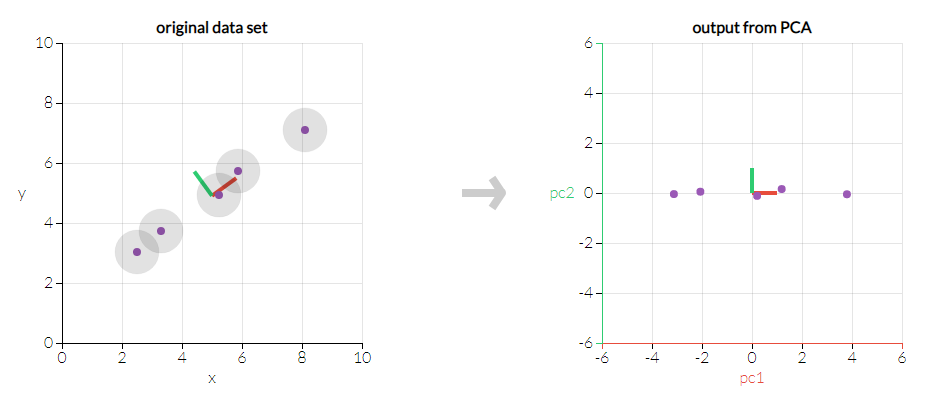
\includegraphics[width=11cm]{images/Segmentierung/PCA}\\
      \tiny{http://setosa.io/ev/principal-component-analysis/}
         \end{tabular}
        
\end{table}
 }
\end{frame}


\begin{frame}[t,fragile]{Bewegungsdetektion mit  PCA}
	\begin{itemize}
 \item Vordergrund- und Hintergrunderkennung
 \begin{itemize}
        \item{Berechnung vom Vordergrund:}
  \item{PCA sucht die ersten k-Hauptkomponenten, die die Daten mit einem maximalen Varianz beschreiben.}
      \end{itemize}

 \item{wobei M das Inputbild und L ist redundante Bildinformation mit Rang-k}
  \end{itemize}
  
\end{frame}


\begin{frame}[t,fragile]{Bewegungsdetektion mit  PCA}
	\begin{itemize}
    \item{Low-Rank Approximation}
\begin{itemize}
    
 \item{Berechne Singulärwertzerlegung aller Bildern im Sequenz X}
 \begin{equation}
\text{SVD(X)}= C = U\Sigma V^T
\end{equation}
 \item{Leite die Matrix ${\Sigma_k}$ von ${\Sigma}$, sodass die ${n - k}$ Werte entlang der Diagonale durch 0 ersetzt werden.}
 \item{Ergibt die Low-Rank Approximation}
\begin{equation}
C_k = U\Sigma_kV^T
\end{equation}

      \end{itemize}
  \end{itemize}
\end{frame}


\begin{frame}[t,fragile]{Bewegungsdetektion mit  PCA}
	\begin{itemize}
 \item Vordergrund- und Hintergrunderkennung
 \begin{itemize}
        \item{Berechnung vom Hintergrund:}
      \end{itemize}


{\large
\begin{equation}
\text{L}=C_1 = U\Sigma_1 V^T
\end{equation}
}
 
  \end{itemize}

  \vspace{0.01em}
  {
\begin{table}
\centering
        \begin{tabular}{cc}
        Originalbild  & Hintergrund \\
        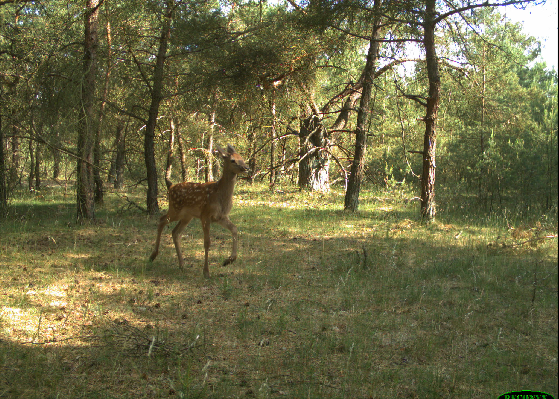
\includegraphics[width=3cm]{images/Segmentierung/original-image}
         &
         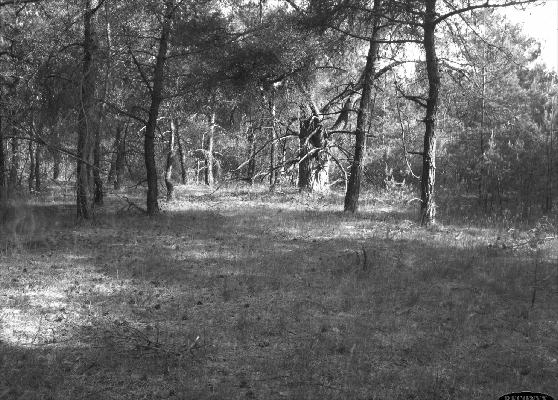
\includegraphics[width=3cm]{images/Segmentierung/background-image}\\
M  & L \\
         \end{tabular}
        
\end{table}
 }
\end{frame}

\begin{frame}[t,fragile]{Bewegungsdetektion mit  PCA}
	\begin{itemize}
 \item Vordergrund- und Hintergrunderkennung
 \begin{itemize}
        \item{Berechnung vom Vordergrund:}
      \end{itemize}
  \end{itemize}

  \vspace{0.01em}
  {
\begin{table}
\centering
        \begin{tabular}{c}
        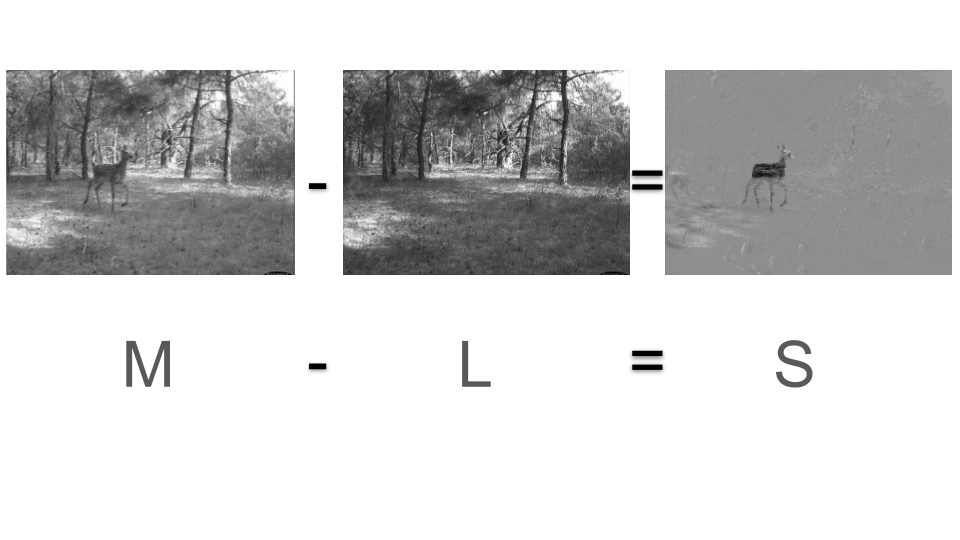
\includegraphics[width=10cm]{images/Segmentierung/foreground-image}
         \end{tabular}
        
\end{table}
 }
\end{frame}

\begin{frame}[t,fragile]{Bewegungsdetektion mit  PCA}
	\begin{itemize}
 \item{Nachbearbeitung vom Vordergrund}
 \begin{itemize}
        \item{Hard- und  Soft Thresholding}
		\item{Aktive Konturen}
		\item{Median- und Gauß-Filterung}
 		\item{Morphologische Operationen}
      \end{itemize}
  \end{itemize}
\end{frame}


\begin{frame}[t,fragile]{Bewegungsdetektion mit  PCA}
	\begin{itemize}
 \item{Nachbearbeitung vom Vordergrund:}
  \end{itemize}
        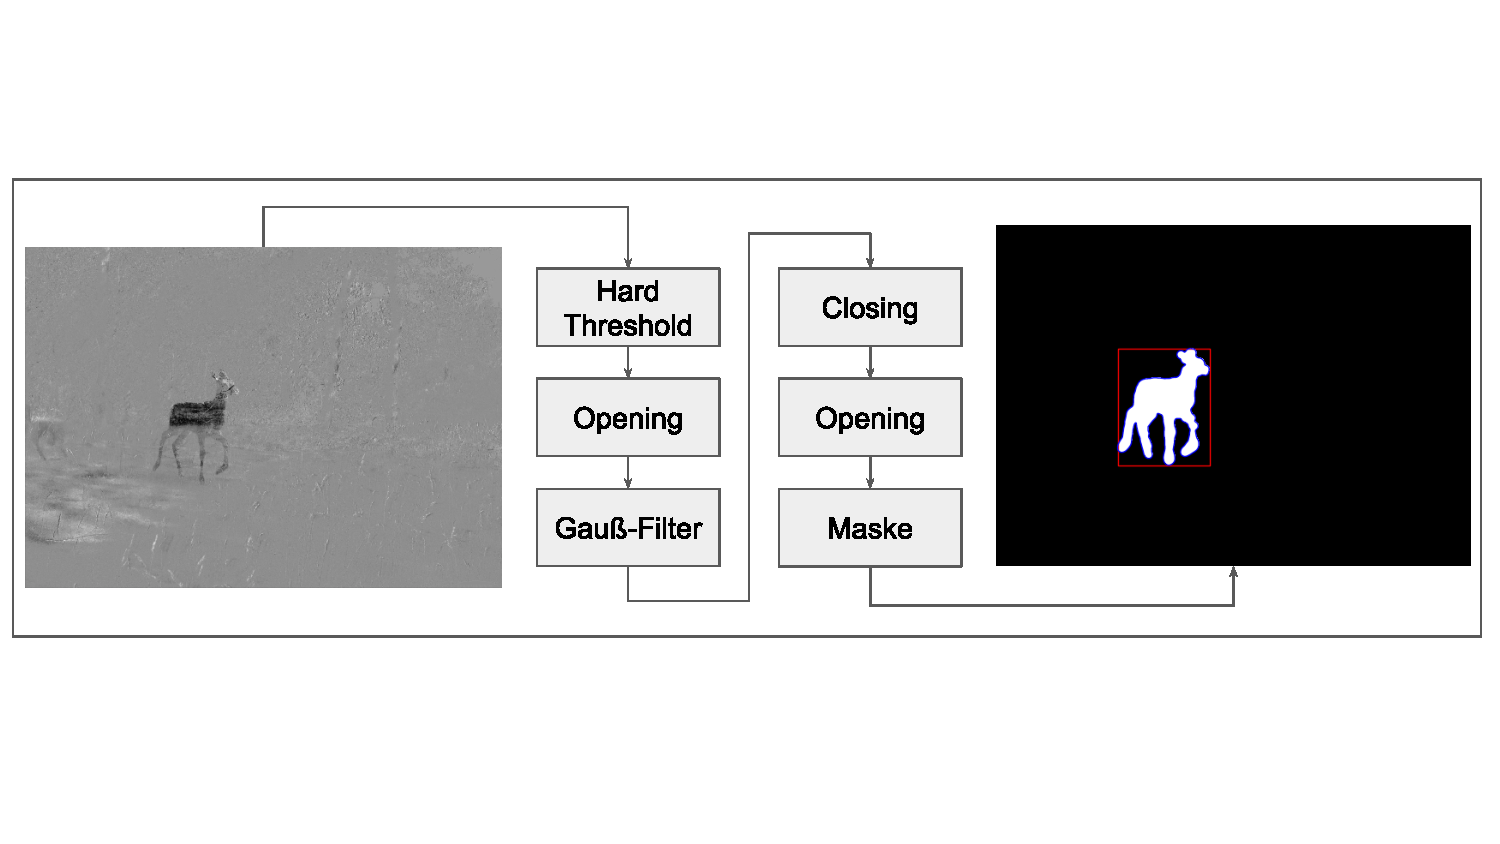
\includegraphics[width=14cm]{images/Segmentierung/pipeline-post2.pdf}

\end{frame}

\begin{frame}[t,fragile]{Objektdetektion mit  PCA}
	\begin{itemize}
 \item{Vorbearbeitung der Daten:}
  \end{itemize}
       
  \vspace{0.01em}
  {
\begin{table}
\centering
        \begin{tabular}{c}
     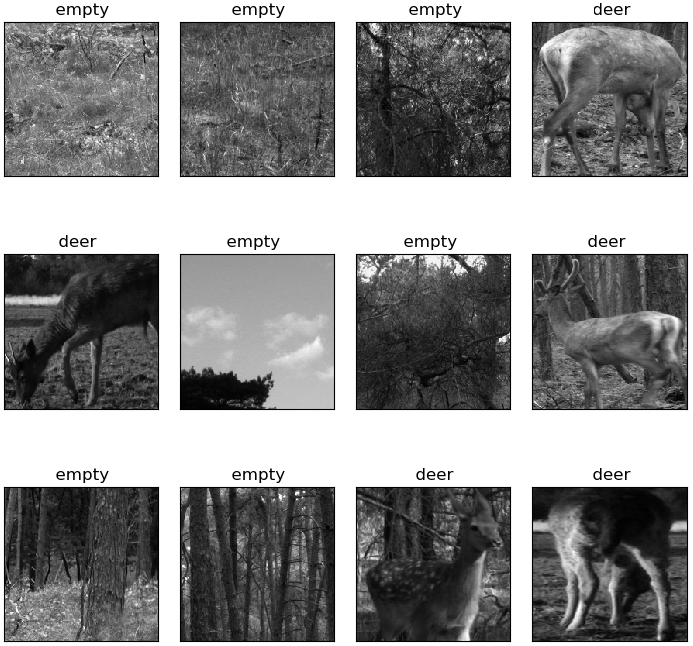
\includegraphics[width=6cm]{images/Segmentierung/data-PCA}
         \end{tabular}
        
\end{table}
 }
\end{frame}

\begin{frame}[t,fragile]{Objektdetektion mit  PCA}
	\begin{itemize}
 \item[1. ]{Daten Zentrieren}
  \end{itemize}
   
  \vspace{0.01em}
  {
\begin{table}
\centering
        \begin{tabular}{c}
        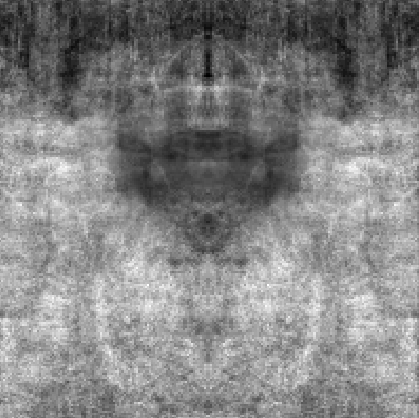
\includegraphics[width=4cm]{images/Segmentierung/PCA-mean}\\
        Mittelwert Bild 
         \end{tabular}
        
\end{table}
 }
\begin{equation}
\text{C} = \text{X} - \bar{\text{x}}
\end{equation}
\end{frame}

\begin{frame}[t,fragile]{Objektdetektion mit  PCA}
\begin{itemize}
 \item[2. ]{Berechne die Eigenwerte und die Eigenvektoren für die Kovarianzmatrix ${CC^T}$:}
  \end{itemize}

   \begin{equation}
\text{SVD}(C) = \text{U} \Sigma V^T 
\end{equation}

	\begin{itemize}
 \item[3. ]{Projektion der Datensatz X in den $r$-Unterraum:}
  \end{itemize}
   \begin{equation}
\text{Y}=\text{U}^{T}_{r}(X-\bar{x})
\end{equation}

\end{frame}


\begin{frame}[t,fragile]{Objektdetektion mit  PCA}
  \vspace{0.01em}
  {
\begin{table}
\centering
        \begin{tabular}{c}
        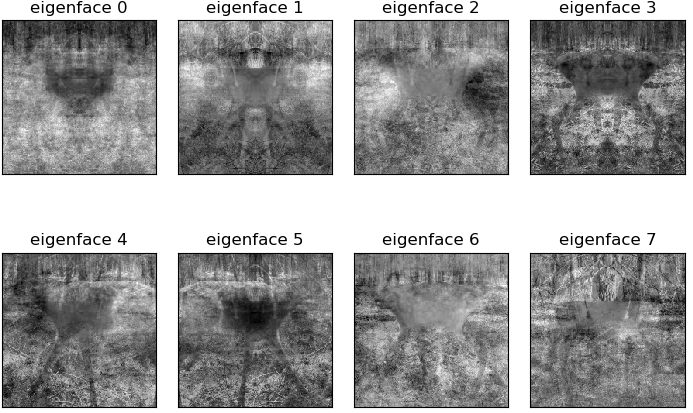
\includegraphics[width=8cm]{images/Segmentierung/pca_eigen}\\
         \end{tabular}
        
\end{table}
 }

\end{frame}

\begin{frame}[t,fragile]{Objektdetektion mit  PCA}
  \vspace{0.01em}
  {
\begin{table}
\centering
        \begin{tabular}{c}
        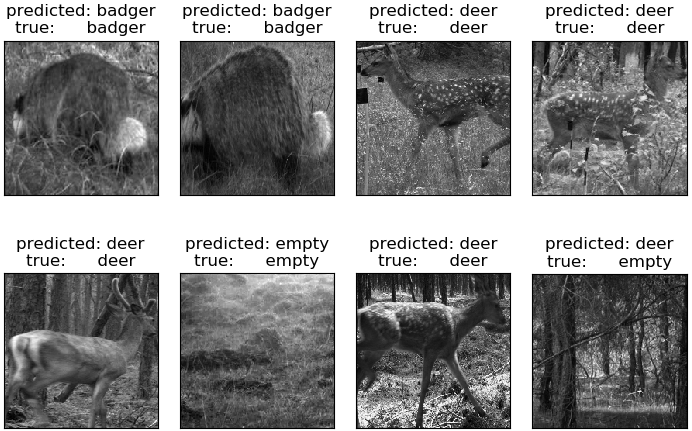
\includegraphics[width=8cm]{images/Segmentierung/pca_test}\\
         \end{tabular}
        \begin{tabular}{ccc}
     				&precision    & recall   \\
		deer   &    0.92  &    0.81\\
		badger   &  0.73   &  1.00\\
		empty     &  0.67   &   0.60\\
         \end{tabular}
\end{table}
 }

\end{frame}

\begin{frame}[t,fragile]{Objektdetektion mit  PCA}

	\begin{itemize}
 \item{Sliding Window}
  \end{itemize}
  \vspace{0.01em}
  {
\begin{table}
\centering
        \begin{tabular}{c}
        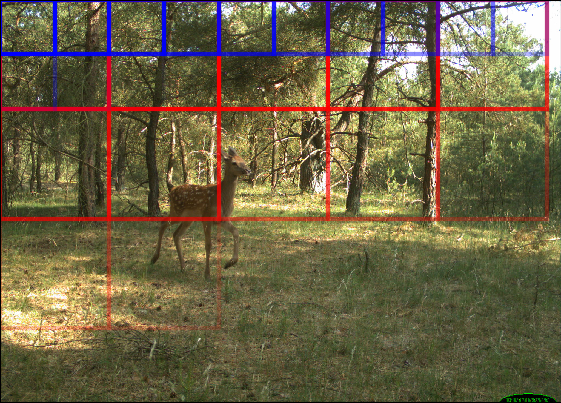
\includegraphics[width=8cm]{images/Segmentierung/sliding.png}\\
         \end{tabular}
\end{table}
 }

\end{frame}


\begin{frame}[t,fragile]{Objektdetektion mit  PCA}
  \vspace{0.01em}
  {
\begin{table}
\centering
        \begin{tabular}{c}
        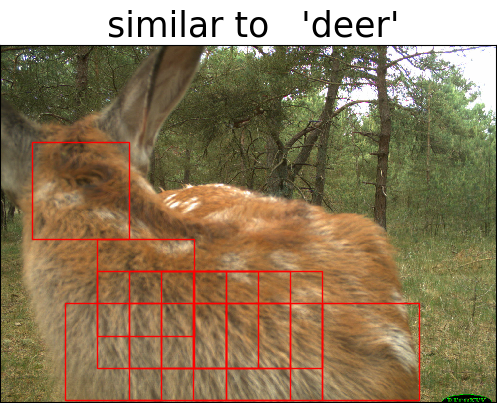
\includegraphics[width=8cm]{images/Segmentierung/seg(1).png}\\
         \end{tabular}
\end{table}
 }

\end{frame}

\begin{frame}[t,fragile]{Objektdetektion mit  PCA}
  \vspace{0.01em}
  {
\begin{table}
\centering
        \begin{tabular}{c}
        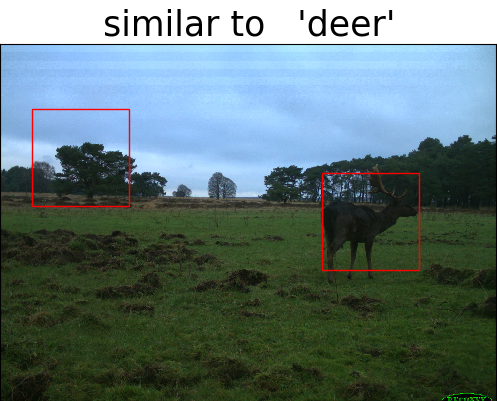
\includegraphics[width=8cm]{images/Segmentierung/seg(2).png}\\
         \end{tabular}
\end{table}
 }

\end{frame}


\begin{frame}[t,fragile]{Objektdetektion mit  PCA}
  \vspace{0.01em}
  {
\begin{table}
\centering
        \begin{tabular}{c}
        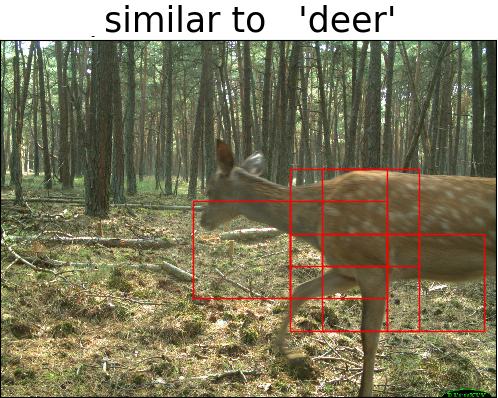
\includegraphics[width=8cm]{images/Segmentierung/seg(3).png}\\
         \end{tabular}
\end{table}
 }

\end{frame}


\begin{frame}[t,fragile]{Objektdetektion mit  PCA}
  \vspace{0.01em}
  {
\begin{table}
\centering
        \begin{tabular}{c}
        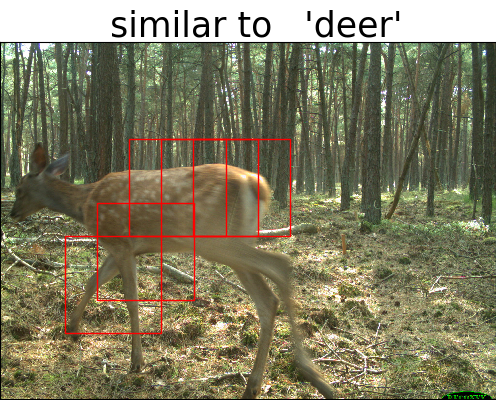
\includegraphics[width=8cm]{images/Segmentierung/seg(4).png}\\
         \end{tabular}
\end{table}
 }

\end{frame}


\begin{frame}[t,fragile]{Objektdetektion mit  PCA}
  \vspace{0.01em}
  {
\begin{table}
\centering
        \begin{tabular}{c}
        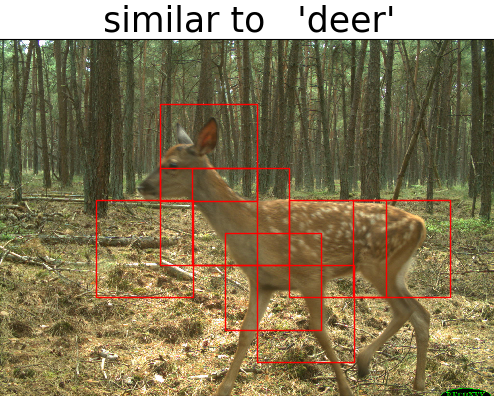
\includegraphics[width=8cm]{images/Segmentierung/seg(5).png}\\
         \end{tabular}
\end{table}
 }

\end{frame}


\begin{frame}[t,fragile]{Objektdetektion mit  PCA}
  \vspace{0.01em}
  {
\begin{table}
\centering
        \begin{tabular}{c}
        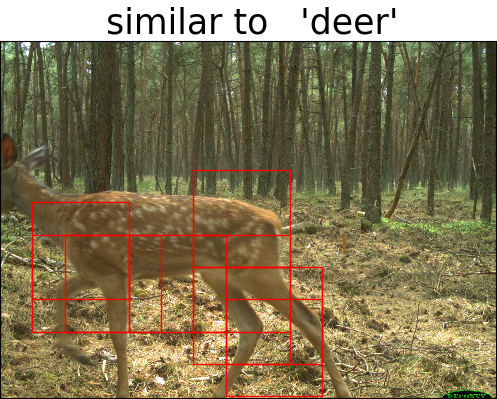
\includegraphics[width=8cm]{images/Segmentierung/seg(6).png}\\
         \end{tabular}
\end{table}
 }

\end{frame}


\begin{frame}[t,fragile]{Objektdetektion mit  PCA}
  \vspace{0.01em}
  {
\begin{table}
\centering
        \begin{tabular}{c}
        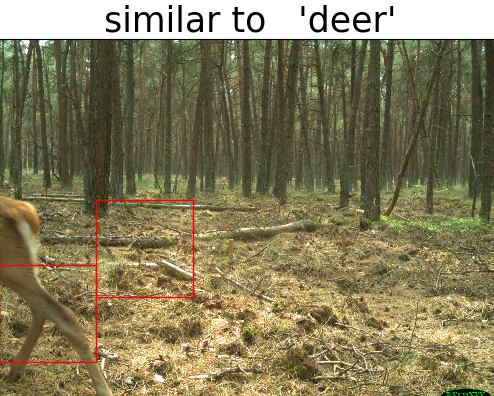
\includegraphics[width=8cm]{images/Segmentierung/seg(7).png}\\
         \end{tabular}
\end{table}
 }

\end{frame}


\begin{frame}[t,fragile]{Objektdetektion mit  PCA}
  \vspace{0.01em}
  {
\begin{table}
\centering
        \begin{tabular}{c}
        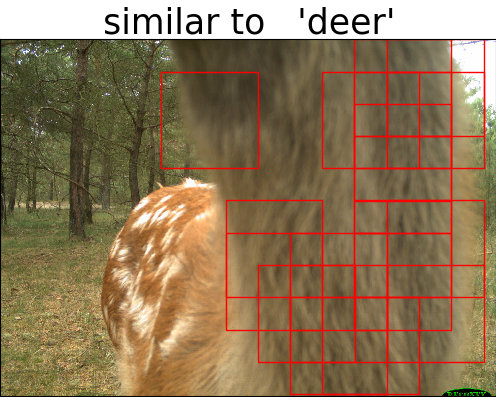
\includegraphics[width=8cm]{images/Segmentierung/seg(8).png}\\
         \end{tabular}
\end{table}
 }

\end{frame}


\begin{frame}[t,fragile]{Objektdetektion mit  PCA}
  \vspace{0.01em}
  {
\begin{table}
\centering
        \begin{tabular}{c}
        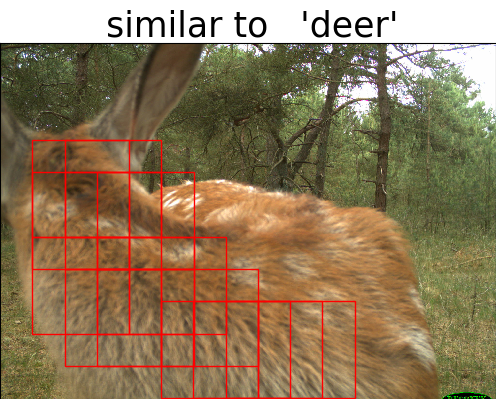
\includegraphics[width=8cm]{images/Segmentierung/seg(9).png}
         \end{tabular}
\end{table}
 }

\end{frame}
